\subsection*{The standard model}

\begin{frame}
\begin{center}
\Large Particle physics?
\end{center}

\vfill

\begin{center}
\Large $\Rightarrow$
study \textbf{elementary particles} and their \textbf{interactions}
\end{center}
\end{frame}

\begin{frame}\def\eDBdir{\homedir/Documents/Enseignement_DB/}
\frametitle{The Standard Model}
\begin{center}
\vspace{-5pt}
\only<1>{\includegraphics[height=\graphh]{\PhDthesisdir/plots_and_images/Particles_tables/steps/01.tex}}%
\only<2>{\includegraphics[height=\graphh]{\PhDthesisdir/plots_and_images/Particles_tables/steps/02.tex}}%
\only<3-4>{\includegraphics[height=\graphh]{\PhDthesisdir/plots_and_images/Particles_tables/steps/03.tex}}%
\only<5>{\includegraphics[height=\graphh]{\PhDthesisdir/plots_and_images/Particles_tables/steps/04.tex}}%
\only<6>{\includegraphics[height=\graphh]{\PhDthesisdir/plots_and_images/Particles_tables/steps/05.tex}}%
\only<7>{\includegraphics[height=\graphh]{\PhDthesisdir/plots_and_images/Particles_tables/steps/06.tex}}%
\only<8>{\includegraphics[height=\graphh]{\PhDthesisdir/plots_and_images/Particles_tables/steps/07.tex}}%
\only<9>{\includegraphics[height=\graphh]{\PhDthesisdir/plots_and_images/Particles_tables/steps/08.tex}}%
\only<10>{\includegraphics[height=\graphh]{\PhDthesisdir/plots_and_images/Particles_tables/steps/09.tex}}%
\vspace{-5pt}
\end{center}

\begin{tikzpicture}[overlay]
\only<2>{
\draw (.35\textwidth, .65\textheight) node [above right] {\Large proton = \quarku\quarku\quarkd};
\draw (.35\textwidth, .65\textheight) node [below right] {\Large neutron = \quarku\quarkd\quarkd};
}
\only<3-4>{
\draw (.35\textwidth, .25\textheight) node [above right] {\Large Beta decay: $\neutron\to\proton+\electron+\nuele$};
\draw (.35\textwidth, .25\textheight) node [below right] {\Large actually $\quarkd\to\quarku+\electron+\antinuele$};
}
\only<4>{
\draw (.6\textwidth, .6\textheight) node {\begin{fmffile}{beta_minus-n_to_p_nu_ele-30x20}%\fmfstraight
\begin{fmfchar*}(30,20)
  \fmfleft{i1,i2,n,i3}
  \fmfright{nu,ele,o1,p}
  \fmf{phantom,tension=4}{n,v1,o1}
  \fmffreeze
  \fmf{fermion, label=\quarkd, l.side=right}{n,v1}
  \fmf{fermion, label=\quarku, l.side=right}{v1,p}
  \fmf{boson, label=$\Wbosonminus$, l.side=right}{v1,v2}
  \fmf{fermion}{nu,v2,ele}
  \fmffreeze
  \fmfi{fermion}{vpath (__n,__v1) shifted (thick*(0,3))}
  \fmfi{fermion}{vpath (__n,__v1) shifted (thick*(0,6))}
  \fmfi{fermion}{vpath (__v1,__p) shifted (thick*(0,3))}
  \fmfi{fermion}{vpath (__v1,__p) shifted (thick*(0,6))}
  \fmffreeze
  \fmfdot{v1,v2}
  \fmflabel{\proton}{p}
  \fmflabel{\neutron}{n}
  \fmflabel{\antinuele}{nu}
  \fmflabel{\electron}{ele}
\end{fmfchar*}
\end{fmffile}
};
}
\end{tikzpicture}
\vspace{-9pt}
\end{frame}

\subsection*{}
\begin{frame}
\begin{center}
\Large

Recherche de bosons de Higgs supplémentaires de haute masse se désintégrant en paire de taus dans l'expérience CMS au LHC à l'aide du \emph{machine learning}

\vfill

Search for additional heavy Higgs bosons decaying to tau lepton pair in the CMS experiment with machine learning techniques
\end{center}
\end{frame}

\subsection*{Beyond the standard model}
\begin{frame}

\begin{center}
Why do we \textbf{search for} additional particles?
\end{center}

\begin{minipage}[c]{.45\textwidth}
\begin{block}{Current standard model status}
\begin{itemize}
\item Robust and predictive (top quark, \Wboson, \Zboson\ and one Higgs boson...)
\item Still not good enough, unable to explain some observations such as:
\begin{itemize}
\item dark matter \only<2>{$\longrightarrow$}
\item matter vs antimatter asymmetry
\item naturalness problem
\item ...
\end{itemize}
\item Go beyond with a new model!
\item Consequences of this new model? \textbf{\color{ltcolorred}Test it!}
\end{itemize}
\end{block}
\end{minipage}
\hfill
\begin{minipage}[c]{.45\textwidth}
\only<2>{\begin{center}
\vspace{\baselineskip}

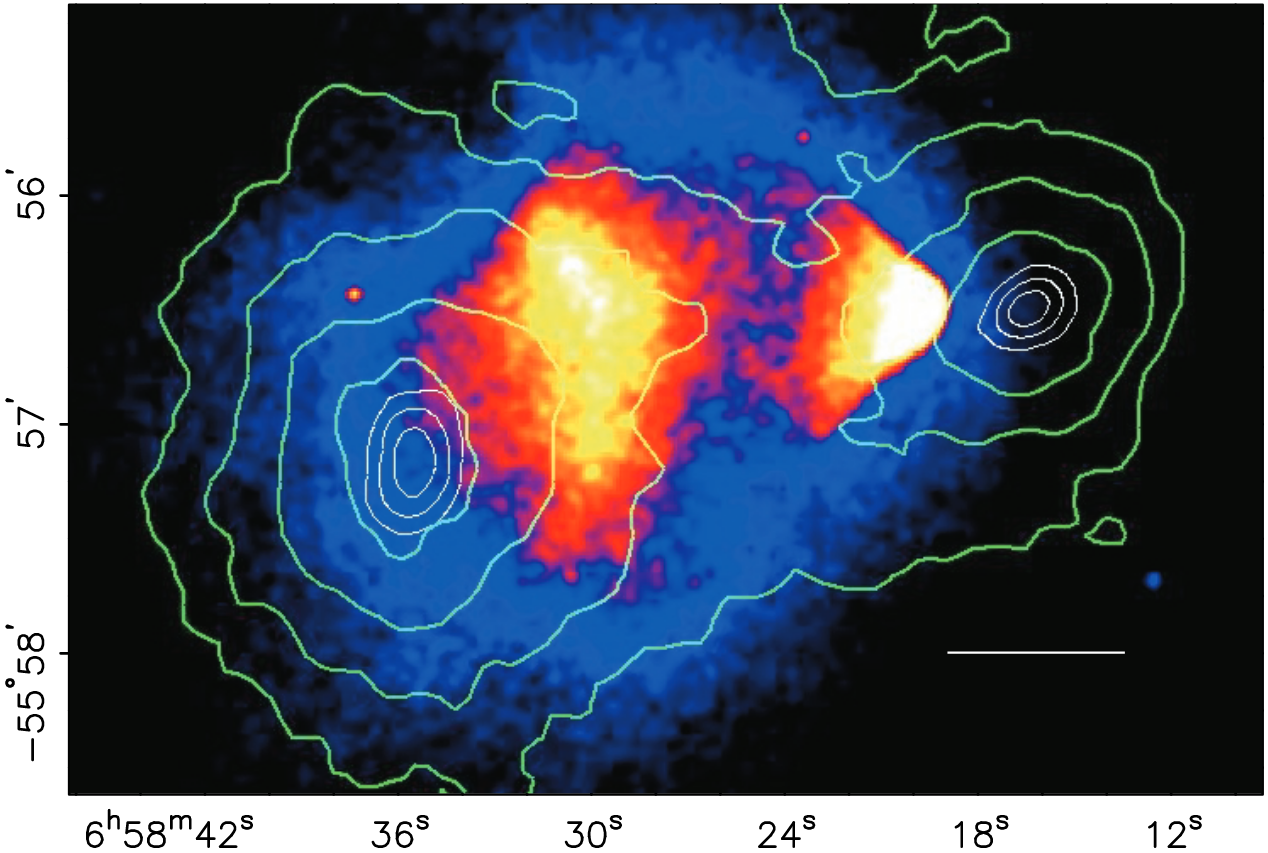
\includegraphics[width=.9\linewidth]{\PhDthesisdir/plots_and_images/from_Clowe_2006/bullet_cluster.png}

Difference due to \textbf{dark matter}!
\end{center}}
\end{minipage}
\beamercite{Clowe_2006}

\begin{tikzpicture}[overlay]
\only<2>{
\draw (.525\textwidth, .65\textheight) node (a) [above right] {Galaxies from:\vphantom{Àq}};
\draw [ltcolorred] (a.east) node [right] (b) {X~rays\vphantom{Àq}};
\draw [ltcolorgreen] (b.east) node [right] (c) {gravitational lensing\vphantom{Àq}};

\draw (.75\textwidth, .45\textheight) coordinate (b1);
\draw (.85\textwidth, .43\textheight) coordinate (b2);
\draw (.7\textwidth, .325\textheight) coordinate (c1);
\draw (.9\textwidth, .44\textheight) coordinate (c2);

\draw [ltcolorred3, thick, -latex] (b) -- (b1);
\draw [ltcolorred3, thick, -latex] (b) -- (b2);
\draw [ltcolorgreen3, thick, -latex] (c) -- (c1);
\draw [ltcolorgreen3, thick, -latex] (c) -- (c2);
}
\end{tikzpicture}
\end{frame}

\begin{frame}{Keywords in title}
\begin{center}
\small
\begin{tikzpicture}
\draw (0,0) node [below right] (t1) {Search for\vphantom{Àq}};
\draw (t1.east) node (t2) [right] {\color{ltcolorblue}\textbf{additional heavy Higgs bosons decaying to tau lepton pair}\vphantom{Àq}};
\draw (t2.east) node (t6) [right] {in the\vphantom{Àq}};
\draw (t6.east) node (t7) [right] {\color{ltcolorred}\textbf{CMS experiment at LHC}\vphantom{Àq}};

\only<2->{
\draw [thick, ltcolorblue] (t2.south east) -- (t2.south west) ;
\draw [thick, ltcolorblue, -latex] (t2.south) --+ (0,-1.5) node (l3) [below] {Part~I\vphantom{Àq}};
\draw  (l3.south) node (l3bis) {\emph{Phenomenology}};
}

\draw (t7.south east) coordinate (0) ;
\only<3->{
\draw [thick, ltcolorred] (t7.south east) -- (t7.south west) ;
\draw [thick, ltcolorred, -latex] (t7.south) --+ (0,-1.5) node (l10) [below] {Part~II\vphantom{Àq}};
\draw  (l10.south) node (l10bis) {\emph{Experimental device}};
}

\only<4->{
\draw ($(l3)!0.5!(l10)$) coordinate (middle);
\draw (middle) + (0, -1.5) node (l12) {Part~III\vphantom{Àq}};
\draw (l12.south) node (l12bis) {\emph{\HAtoTauTau\ analysis}};
\draw [thick, -latex] (l3bis) -- (l12.west) ;
\draw [thick, -latex] (l10bis) -- (l12.east) ;
}

\only<5->{
\draw (l12bis) + (0, -1.5) node {+ Part~IV: \color{ltcolorviolet}\textbf{with machine learning techniques}};
}

\draw (.5\textwidth,-.75\textheight) coordinate (a);
\end{tikzpicture}
\end{center}
\end{frame}